% Этот шаблон документа разработан в 2014 году
% Данилом Фёдоровых (danil@fedorovykh.ru) 
% для использования в курсе 
% <<Документы и презентации в \LaTeX>>, записанном НИУ ВШЭ
% для Coursera.org: http://coursera.org/course/latex .
% Исходная версия шаблона --- 
% https://www.writelatex.com/coursera/latex/5.3

\documentclass[a4paper,14pt]{article}

% Этот шаблон документа разработан в 2014 году
% Данилом Фёдоровых (danil@fedorovykh.ru) 
% для использования в курсе 
% <<Документы и презентации в \LaTeX>>, записанном НИУ ВШЭ
% для Coursera.org: http://coursera.org/course/latex .
% Исходная версия шаблона --- 
% https://www.writelatex.com/coursera/latex/5.3

% В этом документе преамбула

%%% Работа с русским языком
\usepackage{cmap}					% поиск в PDF
\usepackage{mathtext} 				% русские буквы в формулах
\usepackage[T2A]{fontenc}			% кодировка
\usepackage[utf8]{inputenc}			% кодировка исходного текста
\usepackage[english,russian]{babel}	% локализация и переносы
\usepackage{indentfirst}
\frenchspacing

\renewcommand{\epsilon}{\ensuremath{\varepsilon}}
\renewcommand{\phi}{\ensuremath{\varphi}}
\renewcommand{\kappa}{\ensuremath{\varkappa}}
\renewcommand{\le}{\ensuremath{\leqslant}}
\renewcommand{\leq}{\ensuremath{\leqslant}}
\renewcommand{\ge}{\ensuremath{\geqslant}}
\renewcommand{\geq}{\ensuremath{\geqslant}}
\renewcommand{\emptyset}{\varnothing}

%%% Дополнительная работа с математикой
\usepackage{amsmath,amsfonts,amssymb,amsthm,mathtools} % AMS
\usepackage{icomma} % "Умная" запятая: $0,2$ --- число, $0, 2$ --- перечисление

%% Номера формул
%\mathtoolsset{showonlyrefs=true} % Показывать номера только у тех формул, на которые есть \eqref{} в тексте.
%\usepackage{leqno} % Нумереация формул слева

%% Свои команды
\DeclareMathOperator{\sgn}{\mathop{sgn}}

%% Перенос знаков в формулах (по Львовскому)
\newcommand*{\hm}[1]{#1\nobreak\discretionary{}
{\hbox{$\mathsurround=0pt #1$}}{}}

%%% Работа с картинками
\usepackage{graphicx}  % Для вставки рисунков
\graphicspath{{images/}{images2/}}  % папки с картинками
\setlength\fboxsep{3pt} % Отступ рамки \fbox{} от рисунка
\setlength\fboxrule{1pt} % Толщина линий рамки \fbox{}
\usepackage{wrapfig} % Обтекание рисунков текстом
\usepackage{caption}
\usepackage{subcaption}

%%% Работа с таблицами
\usepackage{array,tabularx,tabulary,booktabs} % Дополнительная работа с таблицами
\usepackage{longtable}  % Длинные таблицы
\usepackage{multirow} % Слияние строк в таблице

%%% Алгоритмы
\usepackage[ruled,vlined]{algorithm2e}

%%% Нумерация уравнений
\usepackage{amsmath}

%%% Теоремы
\theoremstyle{plain} % Это стиль по умолчанию, его можно не переопределять.
\newtheorem{theorem}{Теорема}[section]
\newtheorem{proposition}[theorem]{Утверждение}
 
\theoremstyle{definition} % "Определение"
\newtheorem{definition}[theorem]{Определение}
\newtheorem{heuristics}[theorem]{Эвристика}
\newtheorem{corollary}{Следствие}[theorem]
\newtheorem{problem}{Задача}[section]
 
\theoremstyle{remark} % "Примечание"
\newtheorem*{remark}{Примечание}
\newtheorem*{example}{Пример}
\newtheorem*{nonum}{Решение}

%%% Программирование
\usepackage{etoolbox} % логические операторы

%%% Красивые дроби
\usepackage{nicefrac}

%%% Страница
\usepackage{extsizes} % Возможность сделать 14-й шрифт
\usepackage{geometry} % Простой способ задавать поля
	\geometry{top=20mm}
	\geometry{bottom=20mm}
	\geometry{left=20mm}
	\geometry{right=20mm}
 %
%\usepackage{fancyhdr} % Колонтитулы
% 	\pagestyle{fancy}
 	%\renewcommand{\headrulewidth}{0pt}  % Толщина линейки, отчеркивающей верхний колонтитул
% 	\lfoot{Нижний левый}
% 	\rfoot{Нижний правый}
% 	\rhead{Верхний правый}
% 	\chead{Верхний в центре}
% 	\lhead{Верхний левый}
%	\cfoot{Нижний в центре} % По умолчанию здесь номер страницы

\usepackage{setspace} % Интерлиньяж
\onehalfspacing % Интерлиньяж 1.5
%\doublespacing % Интерлиньяж 2
%\singlespacing % Интерлиньяж 1

\usepackage{lastpage} % Узнать, сколько всего страниц в документе.

\usepackage{soul} % Модификаторы начертания

\usepackage{hyperref}
\usepackage[usenames,dvipsnames,svgnames,table,rgb]{xcolor}
\hypersetup{				% Гиперссылки
    unicode=true,           % русские буквы в раздела PDF
    pdftitle={Заголовок},   % Заголовок
    pdfauthor={Автор},      % Автор
    pdfsubject={Тема},      % Тема
    pdfcreator={Создатель}, % Создатель
    pdfproducer={Производитель}, % Производитель
    pdfkeywords={keyword1} {key2} {key3}, % Ключевые слова
    colorlinks=true,       	% false: ссылки в рамках; true: цветные ссылки
    linkcolor=red,          % внутренние ссылки
    citecolor=black,        % на библиографию
    filecolor=magenta,      % на файлы
    urlcolor=cyan           % на URL
}

\usepackage{csquotes} % Еще инструменты для ссылок

%\usepackage[style=authoryear,maxcitenames=2,backend=biber,sorting=nty]{biblatex}

\usepackage{multicol} % Несколько колонок

\usepackage{tikz} % Работа с графикой
\usepackage{pgfplots}
\usepackage{pgfplotstable}

\author{Бычков Андрей}
\title{Квадратизация дифференциальных уравнений}
\date{\today}

%\includeonly{chapters/intro, chapters/ch1}

\begin{document} 

%\maketitle

\tableofcontents

% !TEX root = ../Диплом.tex

\section{Введение}

Динамические системы являются неотъемлемой частью современной прикладной математики. С помощью динамических систем описываются явления в таких областях как физика \cite{physics-example}, химия \cite{chemistry-example}, биология \cite{biology-example}, экономика \cite{economics-example} и многих других. Математические методы позволяют проводить с ними такие операции как упрощение \cite{MOR-book} и анализировать такие их свойства как устойчивость \cite{Strogatz-book} и достижимость \cite{Scott-reachability}. Многие динамические системы, встречающиеся на практике, описываются с помощью нелинейных дифференциальных уравнений. Анализ таких  систем является молодой областью со множеством открытых вопросов, в отличие от анализа линейных систем \cite{MOR-linear-overview}. Поэтому не удивительно, что многие известные методы для работы с нелинейными системами полагаются на аппрокcимацию нелинейных элементов линейными. К сожалению, такой подход часто ведёт к неудовлетворительным результатам. 
Поэтому большой интерес заслужили подходы, целиком полагающиеся на нелинейную природу систем, которыми они оперируют. 
Отдельно выделим метод понижения порядка моделей QLMOR \cite{Gu-PhD, Kramer-Willcox}, который показывает state-of-the-art результаты, сохраняя при этом динамику исходной системы. 
Данный метод полагается на процесс квадратизации --- приведения систем нелинейных дифференциальных уравнений к системе полиномиальных дифференциальных уравнений степени не более двух. 
Примером квадратизации может послужить следующее преобразование (формальное определение и подробные примеры приведены в главах \ref{sec:definitions}, \ref{sec:polynomialization} и \ref{sec:quadratiaztion}):

\[
     \dot x = \frac{1}{1 + e^x} 
\Longrightarrow
\begin{cases}
    \dot x = y_1 \\
    \dot y_0 = y_0 y_1 \\
    \dot y_1 = -y_1 y_2 \\
    \dot y_2 = y_1 y_2 - 2y_2^2
\end{cases}
\]

На данный момент не существует достаточно эффективных или хотя бы реализованных алгоритмов квадратизации --- она всегда совершается вручную.
Из-за этого, даже для сравнительно небольших систем уравнений проводить её крайне долго и сложно. 
Более того, нет гарантий, что полученная квадратизация имеет наименьшую возможную размерность, что критично в задаче понижения порядка моделей. 

В данной работе мы предлагаем алгоритм квадратизации, описываем его реализацию и модификации, и демонстрируем работу реализации на примерах систем из литературы.
% !TEX root = ../Диплом.tex

\section{Цели и задачи}

Цель данной работы --- предложить и реализовать алгоритм нахождения оптимальной квадратизации систем нелинейных дифференциальных уравнений. Эта задача разбивается на следующие подзадачи:

\begin{enumerate}
    \item Формализовать алгоритм квадратизации.
    \item Предложить алгоритмы поиска оптимальной квадратизации.
    \item Реализовать предложенные алгоритмы внутри системе компьютерной алгебры.
    \item Провести эксперименты, чтобы сравнить работу предложенных алгоритмов.
\end{enumerate}

% !TEX root = ../Диплом.tex

\section{Определения и понятия}

\subsection{Системы нелинейных ОДУ, полиномиальные и квадратичные системы}

В данной работе мы рассматриваем системы нелинейных ОДУ вида
\begin{equation} \label{eq:1}
    \begin{cases}
        \dot x_1 = f_1(\vec x)\\
        \vdots\\
        \dot x_n = f_n(\vec x)
    \end{cases},
\end{equation}
где $x_i$ - независимые переменные.

\begin{definition}
    Будем понимать под функциями $f_i(\vec x)$ нелинейные функции, которые могут быть записаны как линейные комбинации элементарных функций $g_k(\vec x)$. Назовём такие функции \textit{нелинейные функции с элементарными нелинейностями}.
    \begin{equation}
        f_i(\vec x) = p_i^T \vec x + a_{i,1} g_1(\vec x) + \cdots + a_{i,m} g_m(\vec x), p_i \in \mathbb{R}^n, a_j \in \mathbb{R}
    \end{equation}
\end{definition}



Таким образом, система \eqref{eq:1} может быть записана в матричной форме

\begin{equation}
    \frac{d}{dt} \vec x = P \vec x + Ag(\vec x)
\end{equation}

где $P^T = [p_1, \cdots, p_n], A = [a_ij], g(\vec x) = [g_1(\vec x), \cdots, g_m(\vec x)]$.

Заметим, что матрица $A$ может получиться крайне разреженной в силу того, что каждое дифференциальное уравнение обычно содержит лишь малую часть функций $g_j(\vec x) \in g(\vec x)$.

Так же, пользуясь тем, что комбинация элементарных функций является элементарной функцией, мы можем покрыть функциями $f$ широкий класс проблем, встречающихся на практике. Мы требуем элементарность функций, так как производная элементарной функции может быть найдена за конечное число шагов, что будет критично для нас в дальнейшем.

\begin{definition}
    Рассмотрим частный случай системы \ref{eq:1}, где функции $f_i$ представляют собой полиномы. Такие системы мы будем называть \textit{полиномиальными}.
\end{definition}

\begin{definition}
    Полиномиальная система имеет порядок $N$, если $N$ - наивысшая степень мономов, образованных переменными $x_i$.
\end{definition}

\begin{definition}
    Полиномиальные системы порядка 2 назовём \textit{квадратичными}
\end{definition}

\subsection{Методы полиномиализации} \label{poly-methods}

\begin{definition}
    Процесс преобразования нелинейных систем \ref{eq:1} к полиномиальному виду будем называть \textit{полиномиализацией}.
\end{definition}

\subsubsection{Полиномиализация с помощью введения алгебраических уравнений} \label{poly-algebraic}

Данный подход заключается в следующем алгоритме:
\begin{enumerate}
    \item Ввести новую переменную $y_i = g_i(\vec x)$, где $g_i(\vec x)$ - неполиномиальная нелинейная элементарная функция.
    \item Заменить $g_i(\vec x)$ на $y_i$ в оригинальном уравнении.
    \item  Добавить новое уравнение $y_i = g_i(\vec x)$ в систему.
\end{enumerate}

Как пример, рассмотрим уравнение $\dot x = x^3 + \frac{1}{1 + x}$. Тогда шаги алгоритма будут выглядеть следующим образом:
\begin{enumerate}
    \item Вводим новую переменную $y = \frac{1}{1 + x}$
    \item Делаем замену в первом уравнении $\dot x = x^3 + y$
    \item  Добавляем новое уравнение в систему $y = \frac{1}{1 + x}\; \Leftrightarrow \; xy + y - 1 = 0$
\end{enumerate}

Получили полиномиальную систему

$\begin{array}{lcl}
    \dot x = x^3 + y \\
    0 = xy + y - 1
\end{array}$
\newline

\begin{remark}
Важно заметить, что данный подход работает для ограниченного класса элементарных нелинейных функций, в частности для рациональных функций. Таким образом мы гарантируем полиномиальность вспомогательных уравнений. В том случае, если мы имеем дело со степенными функциями, логарифмами и многими другими элементарными нелинейностями, например $g_i(x) = e^x$, то получить полиномиальную систему данным методом мы уже не сможем.
\end{remark}


\subsubsection{Полиномиализация с помощью введения дифференциальных уравнений} \label{poly-diff}

Второй подход к полиномиализации предлагает добавление дифференциальных уравнений к системе.
Алгоритм похож на предыдущий за исключением последнего шага:

\begin{enumerate}
    \item Ввести новую переменную $_i = g_i(\vec x)$, где $g_i(\vec x)$ - неполиномиальная нелинейная элементарная функция.
    \item Заменить $g_i(\vec x)$ на $y_i$ в оригинальном уравнении.
    \item Добавить новое уравнение $\dot y_i = \dot g_i(\vec x) = g'_i(\vec x) \dot {\vec x}$ в систему. Данное уравнение получается как сложная производная от $g_i$.
\end{enumerate}
\newline

Таким образом, мы получим систему общего вида

\begin{equation}
    \begin{array}{lcl}
        \dot x_i = p_i^T \vec x + a_{i,1} y_1 + \cdots + a_{i,m} y_m,\quad i = 1, \cdots, n \\
        \dot y_i = \pounds_{\dot{\vec x}} g_i(\vec x) = g'_i(\vec x)(p_i^T \vec x + a_{i,1} y_1 + \cdots + a_{i,m} y_m,),\quad i = 1, \cdots, m
    \end{array},
\end{equation}
\newline
где $g'(\vec x) = \frac {dg(\vec x)}{d \vec x}$, $\pounds_{\dot{\vec x}}$ - производная Ли.

Так как $g'(\vec x)$ состоит только из полиномиальных функций от $x$ и $y_i$, данная система является полиномиальной.

\begin{example}
    Полиномиализуем уравнение $\dot x = sin(x)$. Тогда шаги алгоритма будут выглядеть следующим образом:
    \begin{enumerate}
        \item Избавляемся от $sin(x)$
        \begin{enumerate}
            \item Вводим новую переменную $y_1 =  sin(x)$
            \item Делаем замену в первом уравнении $\dot x = x^3 + y$
            \item Добавляем новое уравнение в систему $\dot y_1 = \dot {sin}(x) = cos(x) \dot x = sin(x) cos(x) = y_1 cos(x)$
            \item Получили систему $\begin{array}{lcl} \dot x = y_1\\ \dot y_1 = y_1 cos(x) \end{array}$
        \end{enumerate}
        \item Избавляемся от $cos(x)$
        \begin{enumerate}
            \item Вводим новую переменную $y_2 =  cos(x)$
            \item Делаем замену во втором уравнении $\dot y_1 = y_1 y_2$
            \item Добавляем новое уравнение в систему $\dot y_2 = \dot {cos}(x) = -sin(x) \dot x = -y_1^2$
        \end{enumerate}
    \end{enumerate}
    
    Получили полиномиальную систему
    
    $\begin{array}{lcl}
        \dot x = y_1\\
        \dot y_1 = y_1 y_2\\
        \dot y_2 = -y_1^2
    \end{array}$
\end{example}



\begin{theorem}
    \begin{enumerate}
    \item Итеративно применяя алгоритмы полиномиализации с помощью введения алгебраических и дифференциальных уравнений, нелинейную систему с элементарными нелинейностями можно привести к полиномиальной форме.
    \item Размер полученной полиномиальной системы является линейным относительно числа элементарных функций в     оригинальной системе.
\end{enumerate}
\end{theorem}

\begin{proof}
    Доказательство первой части уже изложено вместе с алгоритмами полиномиализации.
    
    Рассмотрим вторую часть.
    Заметим, что для того, чтобы избавиться от основной (не композитной) элементарной функции,
    требуется конечное число замен $O(1)$, обычно 1 или 2, например для $sin(x)$.
    
    Для композитных элементарных функций $g(\vec x) = (g_1 \circ g_2 ... \circ g_n)(\vec x)$ необходимо потратить $O(1 \cdot m)$ замен.
    Таким образом, размер полученной полиномиальной системы линеен относительно числа элементарных функций в оригинальной системе.
\end{proof}


\subsection{Методы квадратизации}

\begin{definition}
    Процесс преобразования нелинейных систем \ref{eq:1} к квадратичному виду будем называть \textit{квадратизацией}.
\end{definition}

В данном разделе мы будем рассматривать квадратизации только полиномиальных систем, которые мы уже умеем получать с помощью полиномиализации из систем \ref{eq:1}. Так же заметим, что подходы, применяемые для квадратизации систем, весьма похожи на методы полиномиализации.

\subsubsection{Квадратизация с помощью введения алгебраических уравнений}

Данный подход заключается в следующем алгоритме

\begin{enumerate}
    \item Ввести новую переменную $y_i = m_i(\vec x)$, где $m_i(\vec x) = x_1^{b_1}\cdot \cdots \cdot x_n^{b_n}$ - моном, образованный из переменных системы.
    \item Заменить $m_i(\vec x)$ на $y_i$ в оригинальном уравнении.
    \item Добавить новое уравнение $y_i = m_i(\vec x)$ в систему.
\end{enumerate}

\begin{example}
    Квадратизуем систему, полученную в примере раздела \ref{poly-algebraic}

    $\begin{array}{lcl}
        \dot x = x^3 + y_1 \\
        0 = xy_1 + y_1 - 1
    \end{array}$
    \newline
    
    Теперь проведём квадратизацию
    
    \begin{enumerate}
    	\item Вводим новую переменную $y_2 =  x^2$
    	\item Делаем замену в первом уравнении $\dot x = xy_2 + y_1$
    	\item Добавляем новое уравнение в систему $y_2 - x^2 = 0$
    \end{enumerate}
    
    Получили квадратичную систему
    
    $\begin{array}{lcl}
        \dot x = xy_2 + y_1 \\
        0 = xy_1 + y_1 - 1 \\
        0 = y_2 - x^2
    \end{array}$
\end{example}


\subsubsection{Квадратизация с помощью введения дифференциальных уравнений}

Данный подход заключается в следующем алгоритме:
\begin{enumerate}
    \item Ввести новую переменную $y_i = m_i(\vec x)$, где $m_i(\vec x) = x_1^{b_1}\cdot \cdots \cdot x_n^{b_n}$ - моном, образованный из переменных системы.
    \item Заменить $m_i(\vec x)$ на $y_i$ в оригинальном уравнении
    \item Добавить новое уравнение $\dot y_i = \dot {m_i}(\vec x) = m'_i(\vec x) \dot{\vec x}$ в систему, где $m'(\vec x) = \frac {dm(\vec x)}{d \vec x}$
\end{enumerate}

\begin{example}
    Рассмотрим систему

    $\begin{array}{lcl}
        \dot x = xz^2 + z \\
        \dot z = x \\
    \end{array}$
    \newline
    
    Теперь проведём квадратизацию:
    \begin{enumerate}
        \item Вводим новую переменную $y = z^2$
        \item Делаем замену в первом уравнении $\dot x = xy + z$
        \item Добавляем новое уравнение в систему $\dot y = 2z \dot z = 2xz$
    \end{enumerate}
    
     Получили квадратичную систему
    
    $\begin{array}{lcl}
        \dot x = xy + z \\
        \dot y = 2xz \\
        \dot z = x \\
    \end{array}$
\end{example}


\subsection{Абстрактные синтаксические деревья} \label{AST-section}

Для того, чтобы удобно работать с математическими выражениями, нам понадобится определить на них структуру.
Для этого мы воспользуемся синтаксическим анализом - процессом преобразования последовательности лексем формального языка с его формальной грамматикой.
Результатом обычно является дерево разбора, которое отражает синтаксическую структуру входной последовательности лексем.

В нашем случае мы получаем на вход строковое представление математического выражения, а возвращаем дерево разбора, состоящее из внутренних узлов, представляющий математические функции, например как сложение или взятие логарифма, и листьев, состоящих из переменных и чисел.

\begin{figure}[h!]
    \centering
    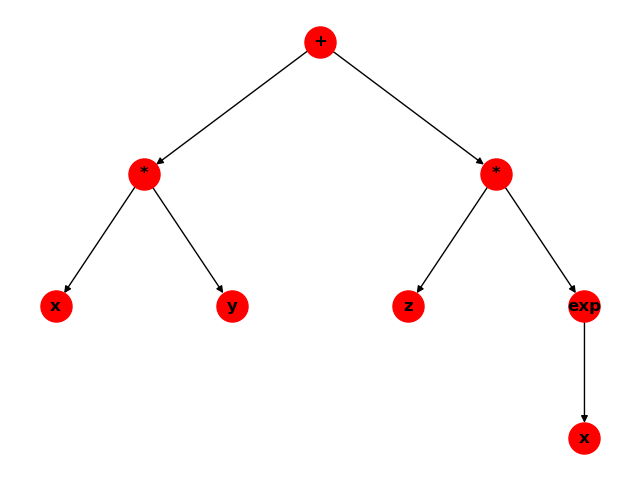
\includegraphics{chapters/images/AST.png}
    \caption{Абстрактное синтаксическое дерево выражения $x \cdot y + z \cdot exp(x)$}
    \label{fig:AST}
\end{figure}

Абстрактное синтаксическое дерево (\textit{АСД}, \textit{AST}) отличается от дерева разбора тем, что в нём отсутствуют узла и рёбра, которые не влияют на семантические свойств выражения. Например, для выражения $3 + 2 \cdot 4$ не нужно расставлять группирующие скобки, так как приоритет операции умножения задан выше, чем приоритет операции сложения.

Многие языки программирования и системы компьютерной алгебры используют данный подход для обработки для обработки своих выражений. В частности, АСД использует фреймворк SymPy \cite{SymPy}, реализованный на языках программирования Python и Julia, который мы будем использовать в дальнейшем.

Оба подхода к полиномиализации, приведённые в пункте \ref{poly-methods}, на первом шаге требуют найти какую-нибудь элементарную нелинейную функцию. Пользуясь средствами синтаксического анализа, мы можем представить правые части системы \ref{eq:1} как абстрактные синтаксические деревья. Таким образом, мы можем свести задачу поиска нужной элементарной функции к задаче поиска на графе. Подробное решение данной задаче находится в пункте \ref{poly-algo}.

\subsection{Граф замен} \label{replacement-graph-section}

Как в процессе полиномиализации, так и в процессе квадратизации, на каждом шаге итерации алгоримта мы выбираем следующую замену переменной. Данный шаг можно обобщить следующим образом.

Граф замен - ацикличный ориентированный граф, чьи вершины представляют системы уравнений, эквивалентные заданной системе, а дуги - преобразования, совершаемые с помощью замены переменной. Входной вершиной мы полагаем заданную систему, а выходной - систему, обладающей нужными нам свойствами.

\begin{wrapfigure}{l}{11cm}
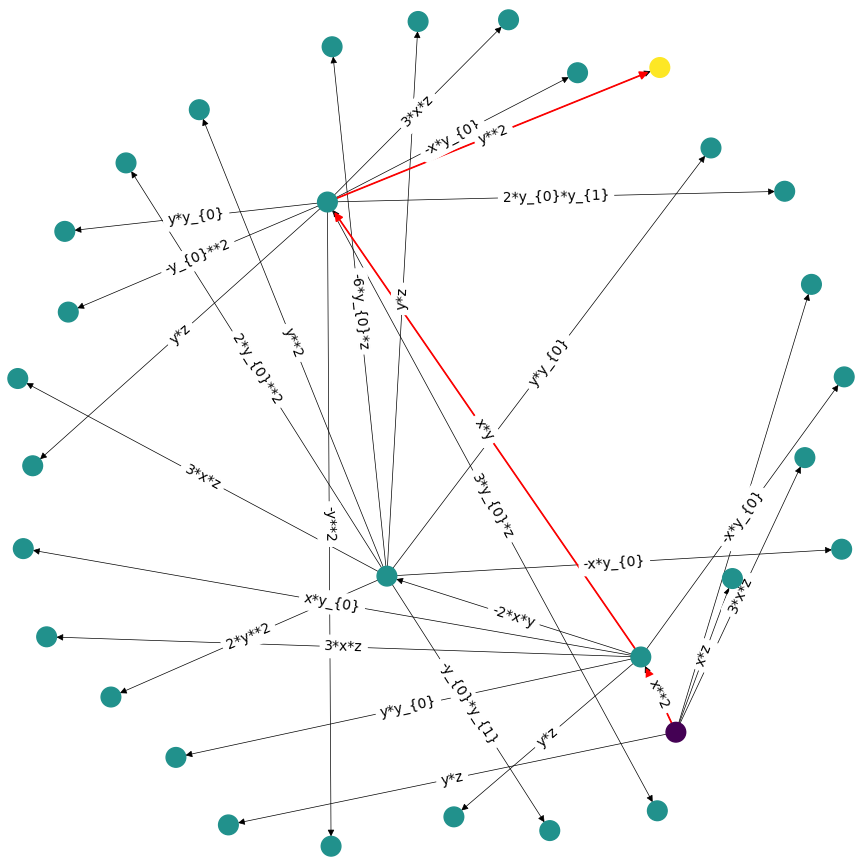
\includegraphics[width=10.5cm,height=10.5cm]{chapters/images/replacement_graph.png} 
\caption{Граф замен}
\label{fig:replacement-graph}
\end{wrapfigure}

Таким образом, мы можем трактовать задачу об оптимальном преобразовании как задачу поиска путей на графе с одним входом и несколькими выходами. Важно заметить, что графы замен, которые нам будут встречаться на практике, часто являются огромными и заранее задан только начальный узел.

В силу того, что квадратизация является гораздо более требовательной к заменам \cite{Gu-PhD}, мы не сможем выбирать замены в произвольном порядке и быстро достичь при этом квадратичной системы. Поэтому мы будет пользоваться алгоритмами поиска на графе замен, что описано в секции \ref{quad-algo}

\subsection{Алгоритмы поиска на графе} \label{search-algo}

В данном разделе мы рассмотрим основные алгоритмы поиска на графе. Подчеркнём, что сам путь нас не интересует, поэтому мы приводим алгоритмы поиска пути на графах, которые, в связи с этим упрощаются.

Пусть $G$ - ориентированный граф, $V$ - множество его рёбер, $E$ - множество его дуг.

\subsubsection{Поиск в глубину (DFS)} \label{DFS-algo}

Поиск в глубину (depth-first search, DFS) заключается в том, что, начиная со стартового узла, исследует его ветви как можно дальше, далее переходя к исследованию других ветвей. Несмотря на то, поиск в глубину применяется в основном при анализе достижимости, он, тем не менее, может находить путь из одной вершины в другую, пусть и не гарантируется то, что найденный путь будет кратчайшим.

\begin{algorithm}[H]
\SetAlgoLined
\SetKwFunction{FDFS}{DFS}
\SetKwProg{Fn}{Function}{:}{}
\KwData{G - входной граф \\
    prop - свойство, которым должна обладать выходная вершина \\
    visited - массив, хранящий для каждой вершины бит, показывающий, посещали ли мы эту вершину}
\KwResult{Вершина, обладающая свойством prop или null, если вершина не найдена}

\Fn{\FDFS{G, v, prop}}{
    visited[v] = true\;
    \If{v обладает свойством prop}{
        \Return v\;
    }
    \ForEach{w: сосед v}{
        \If{visited[w] == false}{
            \Return \FDFS(G, w, prop)\;
        }
    }
    \Return null\;
}
\caption{Поиск в глубину}
\label{algo:DFS}
\end{algorithm}

В худшем случае DFS найдёт искомую вершину последней, поэтому худшая оценка числа операций:
\begin{enumerate}
    \item Чтобы пометить каждую вершину в начале мы посещаем ровно $|V|$ вершин.
    \item В худшем случае мы пройдём по всем дугам графа $|E|$.
\end{enumerate}

Таким образом, число операций в худшем случае можно оценить как $O(|V| + |E|)$

Среднее время работы уже зависит от \textit{prop}.

\subsubsection{Поиск в ширину (BFS)} \label{BFS-algo}

В поиске в ширину (breadth-first search, BFS) граф разбивается на слои: сама входная вершина, вершины на расстоянии 1 от входной вершины, вершины на расстоянии 2 и так далее. Сам поиск исследует слои по возрастанию глубины, пока не найдёт искомую вершину. В отличие от поиска в глубину, BFS всегда отыскивает кратчайший путь до неё.

\begin{algorithm}[H]
\SetAlgoLined
\SetKwFunction{FBFS}{BFS}
\SetKwProg{Fn}{Function}{:}{}
\KwData{G - входной граф \\
    prop - свойство, которым должна обладать выходная вершина \\
    visited - массив, хранящий для каждой вершины бит, показывающий, посещали ли мы эту вершину}
\KwResult{Вершина, обладающая свойством prop или null, если вершина не найдена}

\Fn{\FBFS{G, v_{start}, prop}}{
    \tcc{Очередь из одного элемента}
    Q = \{v_{start}\}\;
    \While{Q не пуста}{
        v = Вытолкнуть(Q)\;
        visited[v] = true\;
        \If{v обладает свойством prop}{
            \Return v\;
        }
        \ForEach{w: сосед v}{
            \If{visited[w] == false}{
                Вставить(Q, w)\;
            }
        }
     }
     \Return null\;
 }
\caption{Поиск в ширину} \label{algo:BFS}
\end{algorithm}

Оценим время работы алгоритма в худшем случае.
\begin{enumerate}
    \item Мы посещаем каждую вершину дважды: в том время, когда мы её помещаем, и при вставке её в очередь: $2|V|$
    \item Каждое ребро в фунции BFS просматривается ровно 1 раз: $|E|$
\end{enumerate}

Таким образом получим оценку $O(|V| + |E|)$, как и у поиска в глубину.

Так же, можно получить альтернативную оценку как числа шагов, так и пространственную сложность в виде $O(b^{d})$, где $b$ - средний коэффициент ветвления графа, $d$- глубина на которой находится выходная вершина. Пусть мы обычно и не знаем $b$ и $d$ точно, но, зная их примерные оценки, мы можем пользоваться данным методом оценки для заранее неисследованных графов.

\subsubsection{Поиск с ограничением глубины (DLS)} \label{DLS-algo}

Поиск с ограничением глубины (depth-limited search, DLS) - вариант поиска в глубину, для которого определяется конечная глубина l на которую он может опуститься. Таким образом, алгоритм всегда работает конечное число шагов, в отличие от DFS, однако ответ не может быть найден, если глубина выходного узла d > l.

\begin{algorithm}[H]
\SetAlgoLined
\SetKwFunction{FDLS}{DLS}
\SetKwProg{Fn}{Function}{:}{}
\KwData{G - входной граф \\
    prop - свойство, которым должна обладать выходная вершина \\
    visited - массив, хранящий для каждой вершины бит, показывающий, посещали ли мы эту вершину \\
    l - предельная глубина}
\KwResult{Вершина, обладающая свойством prop или null, если вершина не найдена}

\Fn{\FDLS{G, v, prop, depth, l}}{
    visited[v] = true\;
    \If{v обладает свойством prop}{
        \Return v\;
    }
    \ForEach{w: сосед v}{
        \If{visited[w] == false \& depth < l}{
            \Return \FDFS(G, w, prop, depth + 1, l)\;
        }
    }
    \Return null\;
}
\caption{Поиск с ограничением глубины} 
\label{algo:DLS}
\end{algorithm}

В худшем случае, число шагов алгоритма оценивается как $O(b^l)$, а пространственная сложность как $O(b \cdot l)$. Таким образом, мы получили лучшие оценки, чем для BFS, при условии, что конечная l выбрана правильно. Гарантировать это поможет следующий алгоритм.

\subsubsection{Поиск в глубину с итеративным углублением (ID-DFS)} \label{ID-DFS-algo}

Поиск в глубину с итеративным углублением (iterative-deepening depth-first search, ID-DFS) запускает DLS на каждой своей итерации и, в случае неудачи, увеличивает конечную глубину l.

\begin{algorithm}[H]
\SetAlgoLined
\SetKwFunction{FIDDFS}{IDDFS}
\SetKwFunction{FDLS}{DLS}
\SetKwProg{Fn}{Function}{:}{}
\SetKwRepeat{Do}{do}{while}
\KwData{G - входной граф \\
prop - свойство, которым должна обладать выходная вершина}
\KwResult{Вершина, обладающая свойством prop или null, если вершина не найдена}

 \Fn{\FIDDFS{G, v_{start}, prop}}{
    l = 1\;
    
    \Do{v == null}{
        v = \FDLS{G, v, prop, 1, l}\;
        l += 1\;
    }
    \Return v\;
 }
\caption{Поиск в глубину с итеративным углублением}
\label{algo:ID-DFS}
\end{algorithm}

Оценкой сложности алгоритма является $O(b^d)$ как у поиска в ширину, а пространственная сложность представляет $O(b \cdot d)$ как у поиска с ограничением глубины, что позволяет ID-DFS использовать преимущества обоих походов.

\subsubsection{Эвристический подход к поиску}

Эвристический поиск, он же информированный поиск представляет собой семейство стратегий поиска,
в котором используются знания о конкретной задаче, зачастую позволяя решать задачу поиска гораздо эффективнее.

Знания о задаче формализуются в качестве эвристических функций.
Эвристические функции сравнивают между собой варианты, из которых алгоритм выбирает следующий шаг.

В случае задач поиска на графе, с помощью эвристических функций мы будем сортировать дуги алгоритмов неинформативного поиска.

Приведём эвристические версии алгоритмов неинформативного поиска
\begin{enumerate}
    \item DFS $\rightarrow$ Поиск по первому наилучшему совпадению (best-first search)
    \item Алгоритм Дейкстры $\rightarrow$ Алгоритм A*
    \item ID-DFS $\rightarrow$ Алгоритм А* с итеративным углублением (Iterative deepening A*, IDA*)
\end{enumerate}


Эвристики, которыми мы будем пользоваться для задачи квадратизации, подробно описаны в секции \ref{heuristics}
% !TEX root = ../Диплом.tex

\section{Методы}

Данная секция описывает предложенные алгоритмы квадратизации и полиномиализации. Как для полиномиализации, так и для квадратизации будем рассматривать подходы с добавлением дифференциальных уравнений.

\subsection{Алгоритм полиномиализации} \label{poly-algo}

\subsubsection{Постановка задачи}

Дана система \ref{eq:1}. Найти минимальную полиномиализацию относительно числа введённых дополнительных уравнений.

Для начала перепишем подход из секции \ref{poly-diff} в более формальном виде. Как уже упоминалось в разделе \ref{AST-section}, нам удобно представлять правые части уравнений системы в виде абстрактных синтаксических деревьев. Из таких деревьев мы формируем лес, которые впоследствии мы будем анализировать.

\begin{algorithm}[H]
\SetAlgoLined
\SetKwFunction{FPoly}{Polynomialize}
\SetKwFunction{FGetNonPoly}{GetNonPolynomialItem}
\SetKwFunction{FFindNonPoly}{FindNonPolynomialItem}
\SetKwProg{Fn}{Function}{:}{}
\KwData{System - система вида \ref{eq:1}}
\KwResult{Полиномиализированная система}
\Fn{\FPoly{System}}{
    NewSystem = Копия(System)\;
    
    \tcc{Лес абстрактных синтаксических деревьев}
    Forest = \{\;\}
    
    \tcc{массив меток, где true - данное дерево не содержит неполиномиальных элементов}
    ForestIsPoly = \{\;\}
    
    \ForEach{r: правое уравнение системы}{
        tree = AST(r)\;
        Добавить(Forest, tree)\;
        ForestIsPoly[tree] = false\;
    }
    
    \While{ForestIsPoly содержит false}{
        g = \FGetNonPoly{Forest, ForestIsPoly}\;
        y_{new} = g\;
        \vec x = Переменные(NewSystem)\;
        ДобавитьУравнение(NewSystem, $\dot y_{new} = \frac{d\ g}{d \vec x} \dot {\vec x}$)\;
    }
    
    \Return NewSystem\;
}

\Fn{\FGetNonPoly{Forest, ForestIsPoly}}{
    \ForEach{tree: ForestIsPoly[tree] == false}{
        nonPolyItem = \FFindNonPoly{tree}\;
        \eIf{nonPolyItem $\ne$ null }{
            \Return nonPolyItem\;
        }{
            ForestIsPoly[tree] = true\;
        }
    }
    \Return null\;
}
\caption{Полиномиализация}
\end{algorithm}

\subsubsection{Прямой обход}

Разберём вариант реализации алгоритма FindNonPolynomialItem, который предполагает прямой проход по синтаксическому дереву - от корня к листьям.

\begin{algorithm}[H]
\SetAlgoLined
\SetKwFunction{FFindNonPoly}{FindNonPolynomialItem}
\SetKwProg{Fn}{Function}{:}{}
\KwData{node - узел AST, составленного из правой части уравнения системы \ref{eq:1}}
\KwResult{Неполиномиальный элемент или null, если такой не найдётся}

\Fn{\FFindNonPoly{node}}{
    \If{неПолиномиальнаяФункция(node)}{
        \Return node\;
    }
    
    \ForEach{child: дети node}{
        nonPolyItem = \FFindNonPoly{child}\;
        \If{nonPolyItem $\ne$ null}{
            \Return nonPolyItem\;
        }
    }
    \Return null\;
}

\caption{Прямой обход синтаксического дерева}
\end{algorithm}

\subsubsection{Обратный обход}

Теперь рассмотрим вариант реализации алгоритма FindNonPolynomialItem, который предпоагает обратный проход по синтаксическому дереву - от листьев к корню.

\begin{algorithm}[H]
\SetAlgoLined
\SetKwFunction{FFindNonPoly}{FindNonPolynomialItem}
\SetKwProg{Fn}{Function}{:}{}
\KwData{node - узел AST, составленного из правой части уравнения системы \ref{eq:1}}
\KwResult{Неполиномиальный элемент или null, если такой не найдётся}

\Fn{\FFindNonPoly{node}}{
    \ForEach{child: дети node}{
        nonPolyItem = \FFindNonPoly{child}\;
        \If{nonPolyItem $\ne$ null}{
            \Return nonPolyItem\;
        }
    }
    
    \If{неПолиномиальнаяФункция(node)}{
        \Return node\;
    }
    \Return null\;
}

\caption{Обратный обход синтаксического дерева}
\end{algorithm}

\subsubsection{Сравнение}

Разница в данных подходах заключается в том, как данные алгоритмы работают с композитным функциями $g = g_1 \circ g_2 \circ \cdots \circ g_k$. Прямой обход, наткнувшись на на неполиномиальную композитную функцию, возвращает сразу всё композицию. Обратный же подход, встретив такую функцию, вернёт максимально глубоко вложенный неполиномиальный элемент. 

Если мы рассматриваем полиномиализацию с введением алгебраических уравнений, то нам не столь важно, как сокращается композиция. Однако при подходе с введением дифференциальных уравнений нам приходится считать сложную производную найденного неполиномиального элемента. Вычислять сложные производные больших композиций дорого, поэтому мы постараемся этого избежать, предпочитая обратный обход прямому. 

\subsection{Алгоритм квадратизации} \label{quad-algo}

\subsubsection{Постановка задачи}

Как мы уже упоминали в разделе \ref{replacement-graph-section}, задача оптимальной квадратизации может быть сформулирована как задача поиска на графе замен. А именно, мы хотим найти квадратичную систему, представляющую собой узел графа замен, так, чтобы найденная квадратичная система находилась на минимальном расстоянии от узла исходной вершины.

Далее рассмотрим известные алгоритмы поиска, приведённые в разделе \ref{search-algo}, в контексте текущей задачи.

\subsubsection{BFS и DFS}

Поиск в глубину и поиск в ширину являются базовыми в задаче поиска, нередко оказываясь достаточно эффективными для многих задач. К сожалению, их в чистом виде достаточно применить для нашей задачи. Действительно, глубина всего графа замен может быть близка к бесконечной при неаккуратном выборе замен, что критично для DFS. В случае BFS нам мешает высокий коэффициент ветвления $b$, который, более того, растёт при для каждого последующего уровня глубины. Таким образом, BFS пригоден для практического использования только в том случае, когда искомая система находится на небольшой глубине. 

\subsubsection{DLS и ID-DLS}

В свете недостатоков BFS и DFS, весьма хорошо смотрится алгоритм поиска с ограничением глубины. Данный алгоритм не уходит дальше заданной глубины, что решает проблему DFS и просматривает узлы на желаемой глубине, а не последовательно идя по слоям, как BFS. Таким образом, при удачно выбранной конечной глубине и хорошем выборе замен на каждом шаге, мы сможем решать задачу за сравнительно небольшое число шагов.

Однако, если мы оценили конечную глубину ниже, чем глубину искомой вершины, то решить задачу мы не сможем. Решает эту проблему алгоритм ID-DFS, который представляет собой DLS, который увеличивает свою конечную глубину в том случае, если искомая вершина не найдена. Недостатком ID-DFS является необходмость исследовать граф заново, если на текущий шаг не нашёл нужную систему. Так же, увеличение глубины всегда происходит только на 1, что не всегда является оптимальной стратегией.

Поэтому мы несколько модифицируем ID-DFS, чтобы устранить данные недостатики. Введём новый алгоритм \textit{Поиск с ограничением глубины с итеративным углублением} (\textit{ID-DLS}), который отличается от ID-DFS в следующем:

\begin{enumerate}
    \item Вместо исследования графа заново после неудачной итерации, ID-DLS сохраняет вершины на текущей конечной глубине вместе с их исходящими заменами. В случае неудачного поиска мы сразу начинаем вычислять неисследованные элементы. Платой за это становится удвоенные затраты на память.
    \item Текущая конечная глубина более гибко изменяется за счёт функции $ОбновитьТекущуюКонечнуюГлубину$. Платой за это становится то, что гарантия оптимальности квадратизации ложится на приведённую функцию. Тем не менее, таким образом мы может искать суб-оптимальные решения с погрешностью, также определяемой функцией $ОбновитьТекущуюКонечнуюГлубину$.
\end{enumerate}

\begin{algorithm}[H]
\SetAlgoLined
\SetKwFunction{FIDDLS}{IDDLS}
\SetKwFunction{FDLS}{DLS}
\SetKwProg{Fn}{Function}{:}{}
\SetKwRepeat{Do}{do}{while}
\KwData{G - входной граф \\
v_{start} - входная вершина \\
prop - свойство, которым должна обладать выходная вершина \\
limit - финальная конечная глубина}
\KwResult{Вершина, обладающая свойством prop или null, если вершина не найдена}

 \Fn{\FIDDLS{G, v_{start}, prop, limit}}{
    currentLimit = 1\;
    
    \tcc{В данную очередь помещаются элементы на текущей конечной глубине вместе с их исходящими заменами. Фактически, мы лениво вычисляем вершины со следующего уровня}
    highDepthQueue = \{\ \}\;
    
    \Do{v == null}{
        \If{currentLimit > limit}{
            \Return null
        }
        v = \FDLS{G, v, prop, 1, currentLimit, highDepthQueue}\;
        currentLimit = ОбновитьТекущуюКонечнуюГлубину(currentLimit)\;
    }
    \Return v\;
 }
\caption{Поиск с ограничением глубины с итеративным углублением}
\label{algo:ID-DLS}
\end{algorithm}



\subsubsection{Выбор эвристик} \label{heuristics}

Точкой ветвления алгоритма квадратизация является шаг, на котором мы выбираем, в какой порядке исследовать возможные замены переменных. Таким образом, определим семейство эвристических функций в задаче квадратизации как 

\begin{equation}
    h:\ \mathbb{M} \longrightarrow \mathbb{R},
\end{equation}
где $\mathbb{M}$ - группа мономов, образованных над переменным $\vec x$ системы \ref{eq:1}. 

\begin{heuristics} \label{FF}
    \textit{Frequent-First}, \textit{FF} - эвристика, выбирающая моном, наиболее часто встречающийся в разложениях. Таким образом, замена переменной затронет наибольшее число мономов в системе.
    
    \begin{example}
        Для разложений $(x^2, xy), (xy, y^2, y^3, xy^2, xy^3), (x^2, y^2, xy)$ мы выберем моном $xy$, так как он встречается в трёх разложениях, а остальные не более чем в двух.
    \end{example}
\end{heuristics}

\begin{heuristics} \label{FVC}
    \textit{Free-Variables-Count}, \textit{FVC} - эвристика, выбирающая моном, образованный из наименьшего числа    переменых. Таким образом, в уравнении $y_i = m'(\vec x) \dot{\vec x}$, соответствующем данной замене, будет минимальное число слагаемых.
    
    \begin{example}
        Из мономов $x^2, xy, xyz$ мы выберем $x^2$, имеющий только одну переменную. Покажем ОДУ, образованные данными заменами:
        \begin{enumerate}
            \item $x^2 \longrightarrow \dot w = 2x \dot x$
            \item $xy \longrightarrow \dot w = \dot x y + x \dot y$
            \item $xyz \longrightarrow \dot w = \dot x yz + x \dot y z + xy \dot x$
        \end{enumerate}
    \end{example}
\end{heuristics}

\begin{heuristics} \label{AED}
    \textit{Auxiliary-Equation-Degree}, \textit{AED} - эвристика, выбирающая моном, порождающий уравнение с наименьшей степенью. 
    
    \begin{example}
        Пусть имеем систему со следующим респределение степеней: $degree(\dot x) = 1,\ degree(\dot y) = 2$. Тогда для замен $x^2, xy, y^2$ получим степени уравнений:
        \begin{enumerate}
            \item $x^2 \longrightarrow \dot w = 2x \dot x \longrightarrow 1 + 1 = 2$
            \item $xy \longrightarrow \dot w = \dot x y + x \dot y \longrightarrow max(1 + 1, 1 + 2) = 3$
            \item $y^2 \longrightarrow \dot w = 2y \dot y \longrightarrow 1 + 2 = 3$
        \end{enumerate}
        Из данных замен выберем $x^2$.
    \end{example}
\end{heuristics}

\begin{heuristics} \label{AEQD}
    \textit{Auxiliary-Equation-Quadratic-Discrepancy}, \textit{AEQD} - эвристика, выбирающая моном, чьё порождённое уравнение наименее отличается от квадратичного. Таким образом, замены, порождающие кважратичные уравнения, имеют самый высокий приоритет. 
    
    \begin{example}
        Пусть имеем замены, порождающие следующие уравнения
        \begin{enumerate}
            \item $m_1 \longrightarrow \dot w = x + y^2 + z^3 \longrightarrow 0 + 0 + 1 = 1$
            \item $m_2 \longrightarrow \dot w = x + y^2 + xy + z^3 \longrightarrow 0 + 0 + 0 + 1 = 1$
            \item $m_3 \longrightarrow \dot w = x + y^2 + z^3 + xyz \longrightarrow 0 + 0 +1 + 1 = 2$
        \end{enumerate}
        Таким образом, $m_1$ и $m_2$ имеют одинаковый приоритет, потому что порождённые ими уравнений имеют минимальную степерь 1.
    \end{example}
\end{heuristics}

\begin{heuristics} \label{AEQD}
    \textit{Summary-Monomial-Degree}, \textit{SMD} - эвристика, представляющая развитие идеи FF. Мы вибираем замену, которая максимально понижает степерь системы.
    
    \begin{example}
        Рассмотрим систему
        
        $\begin{array}{lcl}
             \dot x = xy^2 + y^3 \\
             \dot y = xy + x^2 y + 1
        \end{array}$
        \newline
        
        Понижение степени системы для замены $m$ вычисляетя как $N \cdot (degree(m) - 1)$, где $N$ - число мономов в системе, которые нацело делятся на $m$.
        \begin{enumerate}
            \item $y^2 \longrightarrow 2 \cdot (2 - 1) = 2$
            \item $xy \longrightarrow 3 \cdot (2 - 1) = 3$
            \item $y^3 \longrightarrow 1 \cdot (3 - 1) = 2$
        \end{enumerate}
        Получили, что замена $xy$ максимально сильно снижает степень системы.
    \end{example}
\end{heuristics}

\subsubsection{Правило параллелограмма}

Пусть для начальной полиномиальной системы $S$ имеются две замены $m_1$ и $m_2$.

\begin{wrapfigure}{R}{0.8\textwidth}
\begin{subfigure}{.4\textwidth}
  \centering
  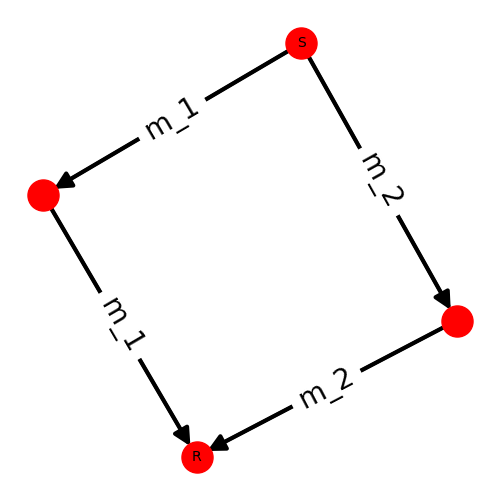
\includegraphics[width=0.8\linewidth]{chapters/images/parallel.png}  
  \caption{Граф замен для $S$}
  \label{fig:parallel-replacement-graph}
\end{subfigure}
\begin{subfigure}{.4\textwidth}
  \centering
  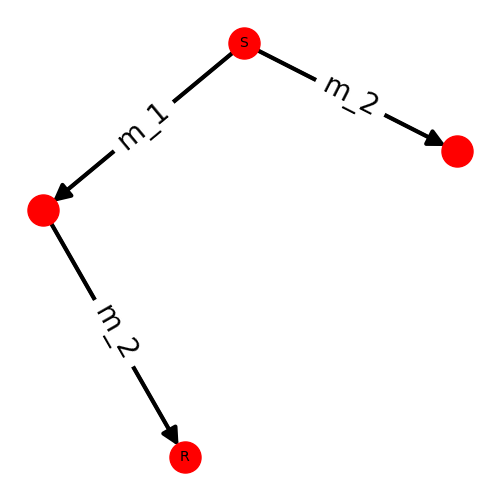
\includegraphics[width=0.8\linewidth]{chapters/images/parallel_red.png}  
  \caption{Упрощённый по правилу параллелограмма граф \ref{fig:parallel-replacement-graph}}
  \label{fig:parallel-replacement-graph-red}
\end{subfigure}
\caption{Правило параллелограмма}
\label{fig:parallel-rule}
\end{wrapfigure}

\begin{proposition}
    Замены $m_1$ и $m_2$ приведут к одной и той же системе $R$ вне зависимости от порядка их проведения. Действительно, ведь в таком случае введённые переменные $y_1$ и $y_2$ получаются перестановкой $[y_1 = y_2,\; y_2 = y_1]$.
\end{proposition}

Таким образом, мы можем убирать часть рёбер из графа во время его исследования. Данная оптимизация становится весьма важна для параллельных версий алгоритма, так как даёт возможность потокам оптимизировать работу друг друга.




% !TEX root = ../Диплом.tex

\section{Эксперименты}

Сравним число шагов, которые понадобятся ID-DLS с разным выбором эвристик, чтобы квадратизировать различные нелинейные системы.



\begin{table}[h!]
\centering
\resizebox{\textwidth}{!}{
\begin{tabular}{||c c c c c c c||} 
     \hline
     Nonlinear system & Random & FF & FVC & AED & AEQD & SMD \\ [0.5ex] 
     \hline\hline
     xSigmoid & 145$\pm$ 85 & 140 $\pm$ 83 & 273 $\pm$ 4 & 146 $\pm$ 77 & 275 $\pm$ 1 & \textbf{52 $\pm$ 31} \\ 
     Rabinovich-Fabrikant & 150 $\pm$ 102 & 142 $\pm$ 88 & 39 $\pm$ 22 & 113 $\pm$ 104 & \textbf{9 $\pm$ 5} & 76 $\pm$ 79 \\
     Blue-sky catastrophe & ? & ? & ? & 12240 $\pm$ 5231 & 1284 $\pm$ 1138 & \textbf{11 $\pm$ 1}  \\
     [1ex] 
     \hline
    \end{tabular}
}
\caption{Сравнение эвристик для ID-DLS}
\label{table:1}
\end{table}

\begin{figure}[h]
\begin{subfigure}{.5\textwidth}
  \centering
  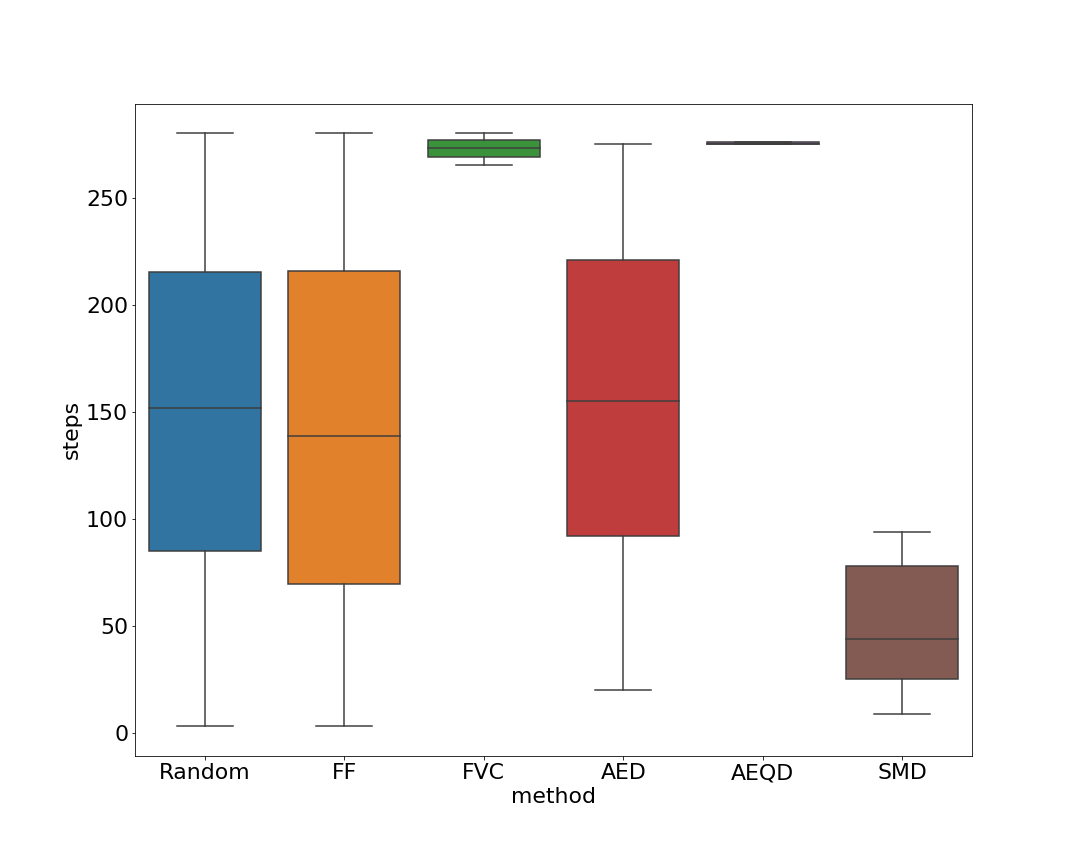
\includegraphics[width=1\linewidth, height=\linewidth]{chapters/images/xSigmoid/box.png}  
  \caption{xSigmoid}
\label{fig:xSigmoid-box}
\end{subfigure}
\begin{subfigure}{.5\textwidth}
  \centering
  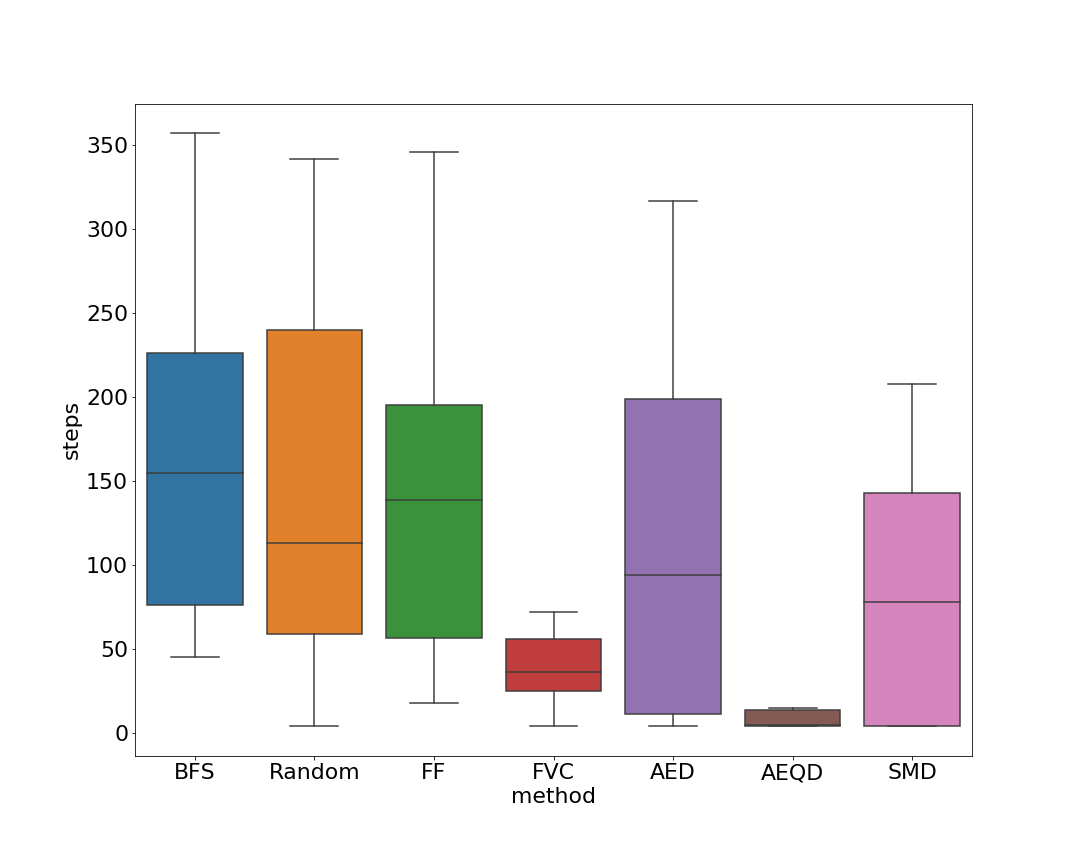
\includegraphics[width=1\linewidth, height=\linewidth]{chapters/images/RabinovichFabricant/4.png}  
  \caption{Rabinovich-Fabrikant}
  \label{fig:Rabinovich-Fabricant-box}
\end{subfigure}
\caption{Сравнение эвристик}
\label{fig:box-plots}
\end{figure}

Таким образом, наиболее успешно показали себя эвристики \textit{AEQD} и \textit{SMD}. Так же \textit{AED} и \textit{FVC} показывают, в целом, результаты лучшие, чем ID-DLS с отсутствием какой либо эвристики. 
% !TEX root = ../Диплом.tex

\section{Заключение}

Существующие алгоритмы полиномиализации и квадратизации не были в достаточной степени формальными, чтобы исполняться на вычислительных устройствах. В данной работе мы предложили формализацию данных алгоритмов на языке графов и свели задачу об оптимальной квадратизации к задаче поиска на графе.

Было показано, какие алгоритмы неинформированного поиска могут справиться с задачей лучше всего. После этого лучший алгоритм был модифицирован до своей эвристической версии. К полученному эвристическому алгоритму был предложен ряд эвристик, после чего было проведено их сравнение. Помимо этого, была проведено разрежение графа, на котором осуществляется поиск, с помощью знаний о предметной области. Таким образом удалось добиться значительного ускорения скорости работы по сравнению с базовыми алгоритмами.

Таким образом, предложенные алгоритмы полиномиализации и квадратизации могут использованы для достаточно быстрого преобразования небольших систем уравнений. Полученный программный пакет, реализованный на языке Python, находится в свободном распространении \cite{QBee}.

Для того, чтобы работать с крупными системами, в будущем будут проведены:
\begin{enumerate}
    \item Оптимизация представления полиномиальных математических выражений, которые могут быть представлены как список кортежей фиксированного размера. Это позволит значительно снизить объём занимаемой памяти и время копирования системы, на данный момент занимающее треть вычислительных ресурсов.
    \item Параллелизация алгоритма квадратизации.
    \item Добавление новых эвристик и синтез уже существующих.
    \item Использование языка программирования Julia. 
\end{enumerate}


\begin{thebibliography}{9}
\bibitem{Gu-PhD} Gu C. Model order reduction of nonlinear dynamical systems : дис. – UC Berkeley, 2011.
\bibitem{Kramer-Willcox} Kramer B., Willcox K. E. Nonlinear model order reduction via lifting transformations and proper orthogonal decomposition //AIAA Journal. – 2019. – Т. 57. – №. 6. – С. 2297-2307.
\bibitem{Harrington-vanGorder} Harrington H. A., Van Gorder R. A. Reduction of dimension for nonlinear dynamical systems //Nonlinear Dynamics. – 2017. – Т. 88. – №. 1. – С. 715-734.
\bibitem{ID-DFS} Korf R. E. Depth-first iterative-deepening: An optimal admissible tree search //Artificial intelligence. – 1985. – Т. 27. – №. 1. – С. 97-109.
\bibitem{physics-example} Blackmore D. L. et al. Nonlinear dynamical systems of mathematical physics: spectral and symplectic integrability analysis. – World Scientific, 2011.
\bibitem{chemistry-example} Karri R. R. Evaluating and estimating the complex dynamic phenomena in nonlinear chemical systems //International Journal of Chemical Reactor Engineering. – 2011. – Т. 9. – №. 1.
\bibitem{biology-example} Jackson T., Radunskaya A. (ed.). Applications of Dynamical Systems in Biology and Medicine. – Springer, 2015. – Т. 158.
\bibitem{economics-example} Lines M. (ed.). Nonlinear dynamical systems in economics. - Springer Science \& Business Media, 2007. - Т. 476.
\bibitem{MOR-book} Schilders W. H. A., Van der Vorst H. A., Rommes J. Model order reduction: theory, research aspects and applications. – Berlin : Springer, 2008. – Т. 13.
\bibitem{Strogatz-book} Strogatz S. H. Nonlinear dynamics and chaos with student solutions manual: With applications to physics, biology, chemistry, and engineering. – CRC press, 2018.
\bibitem{Scott-reachability} Shen K., Scott J. K. Rapid and accurate reachability analysis for nonlinear dynamic systems by exploiting model redundancy //Computers \& Chemical Engineering. – 2017. – Т. 106. – С. 596-608.
\bibitem{MOR-linear-overview} Antoulas A. C., Sorensen D. C. Approximation of large-scale dynamical systems: An overview. – 2001.
\bibitem{SymPy} https://www.sympy.org/ru/index.html

\end{thebibliography}


\end{document} 